\section{Hardware choice} \label{Hardwarechoice}
Hardware components are chosen from the Requirements (see \secref{Requirements}) to build a prototype. 
Some of the hardware components are given with the vehicle (the servo used for steering and the Hall sensors used for velocity measurement) and therefore, aren't described in this section. 
Besides the requirements, the availability of the components and their implementation in the system have to be considered.\todo{What consideration do we have regarding the implementation ?}

%%%%%%%%%%%%%%%%%%%%%%%%%%%%%%%%%%%%%%%%%%%%%%%%%%%%%

\subsection{Microcontroller}
The microcontroller is the brain of the system. The purpose of the microcontroller is to connect all the other hardware components. It also contains the software code necessary to control the rest of the system by sending and receiving electrical signals as needed.

The requirements for the microcontroller are:
\begin{itemize}
\item Have a CPU, that has a frequency greater than \si{XX\ MHz}. \todo{Number}
\item Having I/O connections, both digital and analogue.
\item Having output connections, that can transmit PWM signals.
\item Having 5 free timers,\todo{Where do we have this number from (in the report)?} to run and control the different parts of the system in parallel.
\item Can be powered by an external power source.\todo{?}
\end{itemize}

\subsubsection{Arduino Mega 2560}
The Arduino Mega 2560 is a microcontroller board, which comes with an 8-bit ATmega2560 integrated circuit and extends its I/O ports, see \figref{ArduinoMega} \cite{MegaInfo}. 

\begin{figure}[H]
	\centering
	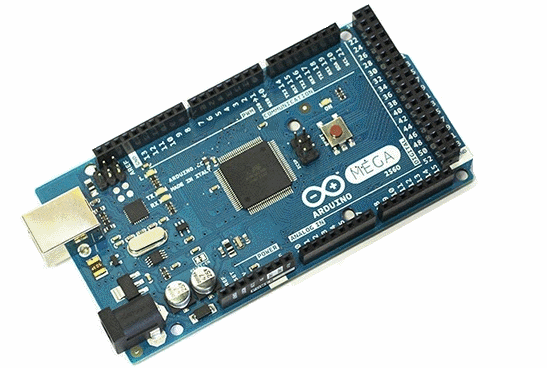
\includegraphics[width=0.5\textwidth]{figures/ArduinoMega.png}
		\caption{An Arduino Mega 2560 board [source: Arduino site]} 
	\label{ArduinoMega}
\end{figure}
%
It has \si{54} digital ports with a 5 volts logic. From these, \si{15} can be used to generate PWM signals. The CPU runs at \si{16 MHz} and the chip has \si{6} integrated timers, one of which is used by the Arduino itself. There are also 4 UARTs, used in serial communication, as well as a setup for SPI communication and an I2C bus. The Arduino can be powered though a USB cable or with an external power source.

The Arduino Mega board is the one that is used in this project, since it ships with all the connections needed to use the already chosen hardware and has many different types of connections to set up the other hardware components. The Arduino is programmable through a serial connection, with the help of avrdude\cite{Avrdude} or simply through the Arduino IDE\cite{ArduinoIDE} which can compile C, C++ and Arduino (syntax very close to C and C++) files.\\
%
By chosing this Arduino microcontroller board as the central hardware component, the rest of them need to be compatible with it.

%%%%%%%%%%%%%%%%%%%-STORAGE-%%%%%%%%%%%%%%%%%%%%%%

\subsection{Storage}
The storage is used for saving the edge map and the route planned for the vehicle. All this data have to be saved from one usage to the other.

The requirements for the storage are:
\begin{itemize}
\item It has to be controlled by the microcontroller.
\item The data shall be retrievable, after a power cut to the storage.
\item It has Have a storage of \si{XX\ MB}. \todo{Number}
\item The transfer speed is greater than \si{XX\ MB/s}. \todo{Number}
\end{itemize}

\subsubsection{SD card} \label{SDcard}
Secure Digital (SD) card is a type of non-volatile flash memory cards. This means that the data will not be lost during a power cut off.\\
%
It comes in various storage sizes, from 1 GB to 2 TB, depending on which type of SD card it is. There is 3 types of SD card, the standard capacity (SDSC), the high capacity (SDHC) and the extended capacity (SDXC). The  difference between the different type, is the file system use on the card and the maximum capacity. With the requirement of a storage size on XX bytes, the SDSC is big enough with a capacity of 2 GB.\\
%
The lowest transfer speed for an SDSC card is \si{2 MB/s}. With the requirement of a transfer speed greater than \si{XX\ bit/s}, the SDSC card is fast enough. 

To use the SDSC card and connect it to the microcontroller, 7 connection pins are required, see \figref{SDcardpinout}. The setup of the SD card is different, depended on which mode is used.

\begin{minipage}{\linewidth}
      \centering
      \begin{minipage}{0.65\linewidth}
			\begin{table} [H]
				\begin{tabular}{|l|l|l|l|}
								
\hline
\textbf{Pin} & \textbf{SPI}  		& \textbf{One bit} 	& 	\textbf{Four bit}  \\
\hline
1			 &	Unused		 		&	Unused			    &	Data 2			   \\
\hline
2			 &	Card Select	 		&	Card Detection		&	Data 3			   \\
\hline
3			 &	Data In		 		&	\begin{tabular}{@{}c@{}} Command \&  \\Response \end{tabular}  &	\begin{tabular}{@{}c@{}} Command \&  \\Response \end{tabular} \\
\hline
4			 &	Power 				&	Power			    &	Power			   \\
\hline
5			 &	Serial clock 		&	Serial clock		&	Serial clock	   \\
\hline
6			 &	Ground		 		&	Ground			    &	Ground			   \\
\hline
7			 &	Data Out	 		&	Data 0			    &	Data 0			   \\
\hline
8			 &	Unused		 		&	Unused			    &	Data 1			   \\
\hline		
				\end{tabular}
				\caption{SD card pinout configuration}							
			\end{table}			
      \end{minipage}
      \hspace{0.03\linewidth}
      \begin{minipage}{0.30\linewidth}
          \begin{figure}[H]
              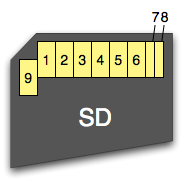
\includegraphics[width=0.95\textwidth]{figures/sdcardpinout}
              \caption{Illustration of a micro size SD card.} % http://elasticsheep.com/2010/01/reading-an-sd-card-with-an-atmega168/
              \label{SDcardpinout}
          \end{figure}
      \end{minipage}
      
  \end{minipage}
  \todo{Talk with niels about table}



The power needed for a SD card is 3.3 volts. There are three possible setups for the SD card: SPI, One-Bit and Four-Bit.
With the SPI setup, the communication between the SD card and the microcontroller is made on two lines. The SPI mode is the most used one for embedded systems.\todo{source !}
With the One-Bit setup, the commands between the SD card and microcontroller are sent on one line and the data is sent though another one.
With the Four-Bit setup, three more data connections are used.\\
%
In this project, the SPI setup is used, as it is the most used method and the extra transfer speed from the Four-Bit setup is not needed. There to have the Arduino 4 pins, that can be set up to SPI communication.\todo{??}\\

The choice for this project is made towards an SDSC card, with a SPI setup, as the capacity and transfer speed meet the requirements. The data will be saved, if the power is cut off. The last requirement, the connections to the microcontroller, is possible since the Arduino Mega 2560 controller contains digital I/O pins, that can be used for the SPI setup of the SD card.

%https://www.sdcard.org/developers/overview/capacity/index.html
%https://www.sdcard.org/developers/overview/speed_class/
%%%%%%%%%%%%%%%%%%%%%%%%%%%%%%%%%%%%%%%%%%%%%%%%%%%%%

\subsection{Motor Driver}
The motor driver is the connection between the microcontroller, the power supply and the motor. The component is used, to separate the low power components, i.e. the microcontroller, and the high power components, i.e. the motor.

The requirements for the motor driver are:
\begin{itemize}
\item Have to be controlled by the microcontroller.
\item Can be powered by an external power source.
\item Can handle up to 7.2 volts.
\item Can power the motor in both direction.
\end{itemize}

\subsubsection{Pololu Dual VNH5019}
The Pololu dual VHN5019 motor driver shield (see \figref{MotorDrive}) is special design to Arduino boards. It can be placed directly atop of the the Arduino, where the pin will connect to the right pins on the Arduino. 

\begin{figure}[H]
	\centering
	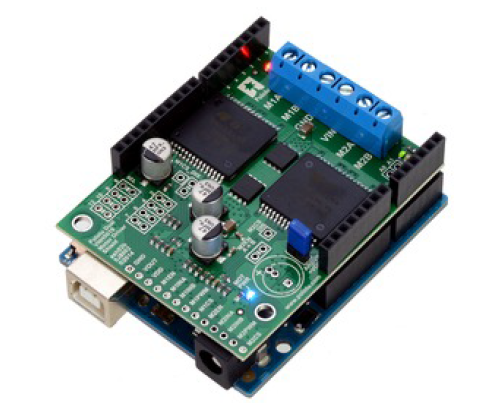
\includegraphics[width=0.50\textwidth]{figures/Motordriver}
		\caption{The motor shield atop of a Arduino Uno.} 
	\label{MotorDrive}
\end{figure}

With the motor shield, it is possible to power the Arduino from a external power source, which also deliver the power to the motor. It is also possible to have the motor shield and the Arduino powered separately. This is determined by a jumper setting on the shield, see \figref{MotorDriveIO}. The motor shield need a power voltage between 7 volts and 12 volts.

\begin{figure}[H]
	\centering
	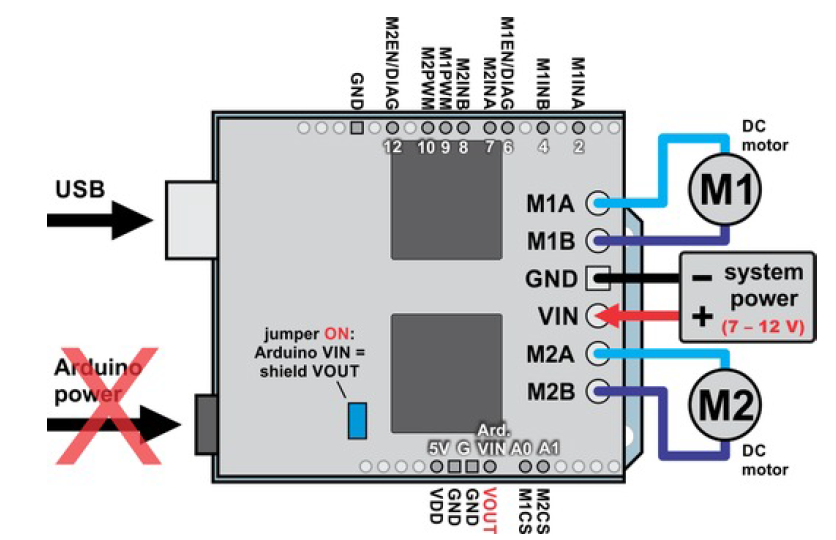
\includegraphics[width=0.60\textwidth]{figures/MotordriverIO}
		\caption{Setup for the mort shield.}
	\label{MotorDriveIO}
\end{figure}

There is two H-bridges on the board, to control two motors. As the project only have one motor, the two H-bridges will be used as one H-bridges. This will give a smaller current through the transistors in the two H-bridges and protect the system.

\begin{figure}[H]
	\centering
	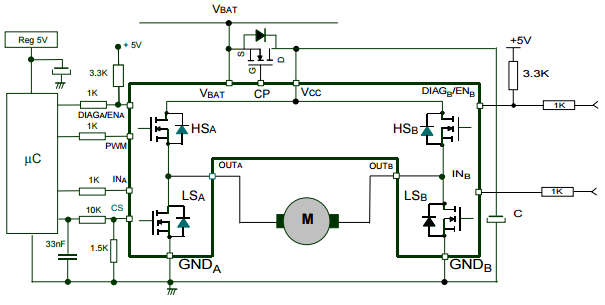
\includegraphics[width=0.85\textwidth]{figures/Hbridges}
		\caption{Illustration of the H-bridge, that the motor shield have two of.}
	\label{Hbridges}
\end{figure}.

Each of the H-bridges is controlled by a PWM signal from the Arduino. But as the H-bridges are used as one, only one will be controlled by a PWM signal. This is done by putting both H-bridges into cruise mode, one to high and the other to ground. Then the PWM signal to the H-bridge, that is set to high, will regulate the voltage sent through the motor. If the voltage have to go reverse through the motor, the settings for the two H-bridges shall swap around.

The Pololu dual VHN5019 motor driver shield will be used in this project, as it is made for the Arduino and therefore easy to implement. There to, it power the Arduino through a external power source and get a high enough power output, in each direction for the motor.

%Source: The datasheet


%%%%%%%%%%%%%%%%%%%%%%%%%%%%%%%%%%%%%%%%%%%%%%%%%%%%%

\subsection{Power Supply}
The external power supply have to both power the motor, which need a high voltage and high power and the other components, which needs low voltage and low power.

The requirements for the power supply are:
\begin{itemize}
\item Voltage output of 7.2 volts.
\item Deliverer a stable power output.
\item Can run the motor at full speed for XX. \todo{Number}
\end{itemize}

\subsubsection{Battery pack}
For the project there will be used a rechargeable battery pack on 7.2 volts. As the prototype is not set to run a long time, less than XX, a normal battery pack used for model vehicles can be used. The battery pack will deliverer a stable power output as long as the power level in the battery pack. In appendix XX \todo{Make test}, it can be seen, that the battery pack can deliverer a stable power output for XX minutes.

%%%%%%%%%%%%%%%%%%%%%%%%%%%%%%%%%%%%%%%%%%%%%%%%%%%%%

\subsection{Wireless communication}
The data from the GOT system is send to the microcontroller with this component. The transmitter will be located at the computer for the GOT system and the receiver on the vehicle. As the prototype will be tested in the control lab, the distance that the wireless communication have to send is less than 10 meters.

The requirements for the wireless communication components are:
\begin{itemize}
\item Have to be controlled by the microcontroller.
\item Have a reach greater than 10 meter. 
\item Powered by an external power supply.
\item The transfer speed is greater than XX bytes per second. \todo{Number}
\item Can be implemented in the GOT code.
\end{itemize}

\subsubsection{Xbee}
Xbee are small radio modules, that is easy to set up. Overview of the Xbee, seen on \figref{XbeeLook} and it pin layout can be seen on \figref{Xbeepinout}.


\begin{minipage}{\linewidth}
	\centering
	\begin{minipage}{0.45\linewidth}      
		\begin{figure}[H]
			\centering
			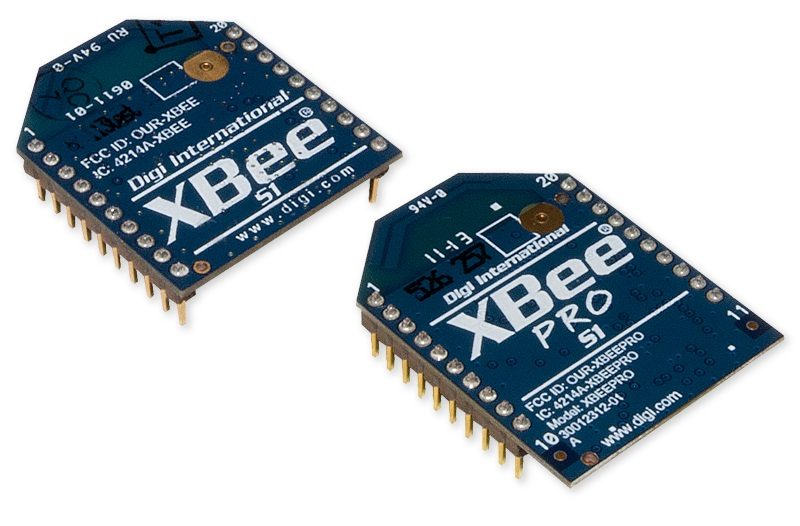
\includegraphics[width=0.95\textwidth]{figures/Xbee}
			\caption{The Xbee radio modules} 
			\label{XbeeLook}
		\end{figure}
	\end{minipage}
	\hspace{0.03\linewidth}
	\begin{minipage}{0.45\linewidth}
		\begin{figure}[H]
			\centering
			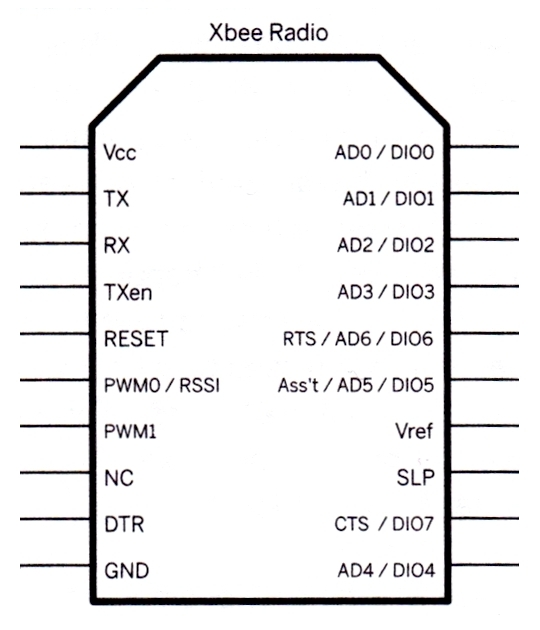
\includegraphics[width=0.95\textwidth]{figures/XbeeIO}
			\caption{Pinout for the Xbee radio modul.} 
			\label{Xbeepinout}
		\end{figure}
	\end{minipage}
\end{minipage}

\todo{Snak med vinkel om at få teksten align}

The Xbee modules communicates through a UART connection (the TX and RX pin). As the Arduino have three UART connections, beside the one use to program the Arduino with, the Xbee can be connected. The software for the GOT system is running on C\# (See in appendix \secref{GoTDescription}) and the computer running the software have some serial port, that can be connected to the software and the Xbee. So the Xbee can be used for the connection between the GOT system and the Arduino.

To run the Xbee modules, there is needed a power on 3.3 volts, a ground and a UART on 3.3 volts. The rest of the pins will not be needed in this project. It have a transfer speed up to 115.2 kilobits per second and have a reach up to 100 meters indoor and 300 meters outdoor. It transmit with 1 millivolt (0 dBm) and can receive downto -96 dBm and transmits at a 2.4 GHz frequency. The Xbee is already ready for communication, with the lower level of communication, the physical layer, already design. A transportation layer can be added to the protocol, to add more error handling and to set up how the data shall be send. \todo{Not sure if that is all the layers}

%http://www.digi.com/products/xbee-rf-solutions/modules/xbee-digimesh-2-4#specifications

%%%%%%%%%%%%%%%%%%%%%%%%%%%%%%%%%%%%%%%%%%%%%%%%%%%%%

\subsection{Angular sensor}
The angular sensor is used in the feedback for the control system.

The requirements for the angular sensor are:
\begin{itemize}
\item Have to be controlled by the microcontroller.
\item Having a sampling frequency greater than XX. \todo{Number}
\item Having a latency smaller than XX. \todo{Number}
\item Powered by an external power supply.
\end{itemize}

\subsubsection{HMC5883L}
On Sparksfun's "9 degrees of freedom" board, there is mounted a magnetometer, the HMC5883L. There will be used a magnetometer as the angular sensor, as the magnetometer can be setup as a compass and give out a angle compared to north. As the direction to north always is the same, the system will not need a new calibration of the angular sensor, if used in a new area. This will have to be needed, if the direction was taken from a local direction point, like a point in the GOT system.

\begin{figure}[H]
	\centering
	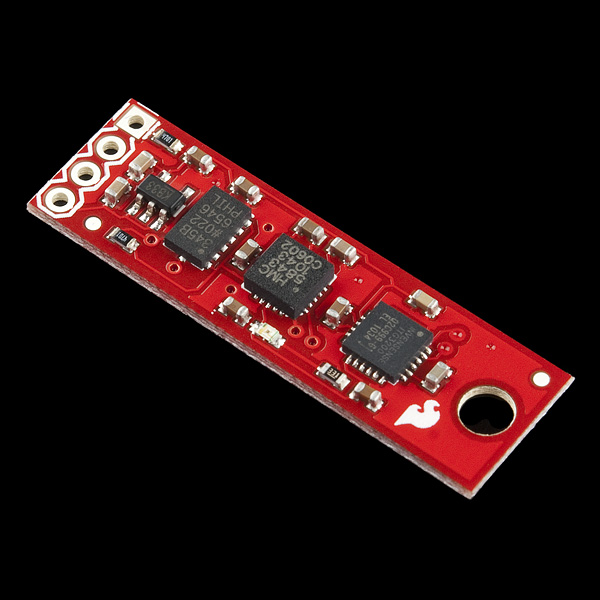
\includegraphics[width=0.50\textwidth]{figures/NineDegree}
		\caption{Sparksfun's "9 degrees of freedom" sensor stick} 
	\label{NineDegree}
\end{figure}

The "9 degrees of freedom" sensor stick, see \figref{NineDegree}, will be used in the project. Beside the magnetometer, there is a accelerometer and a gyroscope on the board, but these will not be used. The "9 degrees of freedom" sensor stick is madded to be used with a micro controller and comes with software to Arduino. It needs a I2C bus to communicated with the Arduino, which the Arduino have one of, which it not in use.

%%%%%%%%%%%%%%%%%%%%%%%%%%%%%%%%%%%%%%%%%%%%%%%%%%%%%

\subsection{Power monitor}
The power monitor is used to give a feedback to the system on the level of power in the battery pack.

The requirements for the angular sensor are:
\begin{itemize}
\item Have to be controlled by the microcontroller.
\item Measure the battery pack voltage output downto 5,7 volt.
\end{itemize}

\subsubsection{Voltage divider}
A voltage divider is a electronic circuit, that divide the input voltage with a constant, that is depending on the values on the resistor, that is used in the circuit, see \figref{VoltDivFig}.

\begin{figure}[h!]
\centering
\begin{circuitikz}
\draw (0,0)
to[V,v=$V_{in}$] (0,2)
to[short] (2,2)
to[R=$R_1$] (2,0)
to[R=$R_2$] (2,-2)
to[short] (0,-2)
to[short] (0,0);
\draw (2,-2) 
to[short] node[ground] {} (2,-3);
\draw (2,0)
to[short] (3,0)
to[short,l=$V_{out}$] (4,0);
\end{circuitikz}
\caption{Standard voltage divider} 
\label{VoltDivFig}
\end{figure}

The output of the voltage divider can be find with \eqref{VoltageDividere}. 

\begin{flalign}
\eq{V_{out}}{\frac{R_2}{R_1 \cdot R_2} \cdot V_{in}}\unit{V} 
\label{VoltageDividere}
\end{flalign}

The input will be set to the battery pack and the output, to a analogue pin on the Arduino. The analogue pin on the Arduino can measure from 0 volts to 5 volts with a accuracy of 10 bits. This gives 1023 steps from 0 to 5 volts and each step is 4,9 millivolts. The size of each step and the interval for the measuring is multiply by the constant from the voltage divider, so it is possible to measure voltage over 5 volts. 
A voltage divider will be used, as it can be scaled to the interval that it have to measure inside. The voltage divider will be connected to a analogue pin on the Arduino, that will make the measurement on the output of the voltage divider.


From the requirements for the system to the hardware parts, these components have been chosen. After have chosen the different hardware components for the prototype, the different components have to be implemented in the system.
%%%%%%%%%%%%%%%%%%%%%%%%%%%%%%%%%%%%%%%%%%%%%%%%%%%%%


%Pins on the arduino
%SD card (4 I/O)
%Xbee (1 TX and 1 RX)
%Hall (2 I/O)
%Angular (1 SDL and 1 SDA)
%Servo (1 PWM)
%Motor (1 PWM)
